
%
% Computational Astrophysics
%

\documentclass{article}

%-------------------------------------------------------------------------------------------------------------
%  package
%--------------------------------------------------------------------------------------------------------------
%版面規劃(a4大小,上下左右距0.9inch)
\usepackage[a4paper,margin=0.9in]{geometry}

%和插入圖片相關的package
\usepackage{graphicx}
\usepackage[FIGTOPCAP]{subfigure}

\usepackage{amsmath,booktabs,threeparttable,url, bm}
%\usepackage[hyphenbreaks]{breakurl}

%連結註腳網頁
\usepackage[colorlinks,linkcolor=blue]{hyperref}

%中文化package
\usepackage{CJKutf8}

%\newcommand{\cntext}{\begin{CJK}{UTF8}{bsmi}\end{CJK}}

\title{Assignment 1 of \\Computational Astrophysics in NTHU}
\author{Wei-Hsiang Yu 游惟翔}


%-------------------------------------------------------------------------------------------------------------
%  文件開始
%--------------------------------------------------------------------------------------------------------------
\begin{document}

\begin{CJK}{UTF8}{bsmi}
%中文化需要加上此行才有title/author/date
\maketitle
\end{CJK}


%-------------------------------------------------------------------------------------------------------------
%  Written Assignments
%--------------------------------------------------------------------------------------------------------------
\section{Written Assignments}

%Q1---------------------------------------------------------------------
\textbf{Q1 : Angry Bird\\}

If we \textbf{ignore air resistance}, the distance R of angry bird moving in horizontal direction will be Eq.\ref{eq:Rno}.
\begin{equation}
    R = \frac{v_{0y}^2\sin{2\theta}}{g}
    \label{eq:Rno}
\end{equation}

So I think the error will come from $\sin{\theta}=x-\frac{\theta^3}{3!}+\frac{\theta^5}{5!}-\frac{\theta^7}{7!}+...$
and gravity constant g=9.8....., because there will be calculated by approximation.\\

And then, I consider projectiles \textbf{with air resistance} $F_{D}=cv^2$, we can do two orthogonal coordinates analysis:
\begin{equation}
    y = v_{0y}t-\frac{1}{2}(g+\frac{c(v_{0y})^2}{m})t^2
    \label{eq:yposition }
\end{equation}
\begin{equation}
    x = v_{0x}t-\frac{1}{2}(\frac{c(v_{0x})^2}{m})t^2
    \label{eq:xposition}
\end{equation}

When a bird hit the ground, i.e. $y=0$, Eq.\ref{eq:yposition }. can be written as:
\begin{equation}
    t =\frac{2mv_{0y}}{mg+c(v_{0y})^2}
    \label{eq:time}
\end{equation}

So during time t, angry bird fly distance R, we substitute Eq.\ref{eq:time}. into Eq.\ref{eq:xposition} to get R'.
\begin{equation}
    R' =\frac{2mv_{0x}v_{0y}}{mg+c(v_{0y})^2}
    -\frac{1}{2}\frac{4mv_{0x}^2v_{0y}^2}{(mg+c(v_{0y})^2)^2}=
    \frac{mv_{0}^2\sin{2\theta}}{mg+c(v_{0}\sin{\theta})^2}-
    \frac{1}{2}\frac{mv_{0}^4(\sin{2\theta})^2}{(mg+c(v_{0}\sin{\theta})^2)^2}
    \label{eq:R}
\end{equation}

In this condition, because air resistance need to consider bird's mass m, and the mass is not given, so m need to be assumed. Air resistance coefficient is another variable need to be assumed, since it is relative to bird's cross-section area.

About approximations and possible errors, I think it is like the condition of projectile ignore air resistance. The function $\sin{\theta}$ will make calculation have error.
\\ \\

%Q2---------------------------------------------------------------------
\textbf{Q2 : forward error \& backward error\\}

For question number 2, the problem told us that:

\begin{equation}
    y=f(x)=\cos (x)=1-\frac{x^2}{2!}+\frac{x^4}{4!}-\frac{x^6}{6!}+...
    \label{eq:1}
\end{equation}
\begin{equation}
    \hat{y}= 1-\frac{x^2}{2!}
    \label{eq:2}
\end{equation}


Forward error will be the error between Eq.\ref{eq:1}. \& Eq.\ref{eq:2}. ,i.e.
\begin{equation}
Forward error : \left|\hat{y}-y\right| = -\frac{x^4}{4!}+\frac{x^6}{6!}+...
\label{eq:3}
\end{equation}

Backward error will be the error $\triangle x$ of variable we give into the function.
\begin{equation}
    1-\frac{x^2}{2!}+\frac{x^4}{4!}-\frac{x^6}{6!}+...=y=\hat{y}(x+back error)=1-\frac{(x+\triangle x)^2}{2!}
    \label{eq:4}
\end{equation}

After we elimination equation, we can get the relation of $\triangle x$ :
\begin{equation}
    2x\triangle x +\triangle x^2 = 2(\frac{x^4}{4!}-\frac{x^6}{6!}+...)
    \label{eq:5}
\end{equation}

The question give us the condition number for $x=1$. So we can use this condition into Eq.3 \& Eq.5. to acquire the forward error = 0.0403 ;backward error = 0.03952\\ \\
%Q3---------------------------------------------------------------------
\textbf{Q3 : Simulate all stars in our Milky Way}

I search the internet and find
\footnote{space demand of fortran data type, in page 3
\href{https://jupiter.math.nctu.edu.tw/~smchang/fortran/fortran90.pdf}{https://jupiter.math.nctu.edu.tw/~smchang/fortran/fortran90.pdf}}
: a real number, which is with 4 kind, will spend 4 bytes(32 bits) space in our computer.

The problem say that we have 250 billion$(*10^9)$stars in our Milky Way, and each stars need to record 10 variables.So we can calculate the total space we need to use is

$$    4(bytes)*10(variables)*250*10^9(number of stars)=1* 10^{13}(bytes)=10(TB) $$


%-------------------------------------------------------------------------------------------------------------
%  Programming Assignments
%--------------------------------------------------------------------------------------------------------------
\section{Programming Assignments}


%Q1---------------------------------------------------------------------
\textbf{Q1 : git\\}
\begin{figure}[h]
    \centering
    \subfigure[github]{
        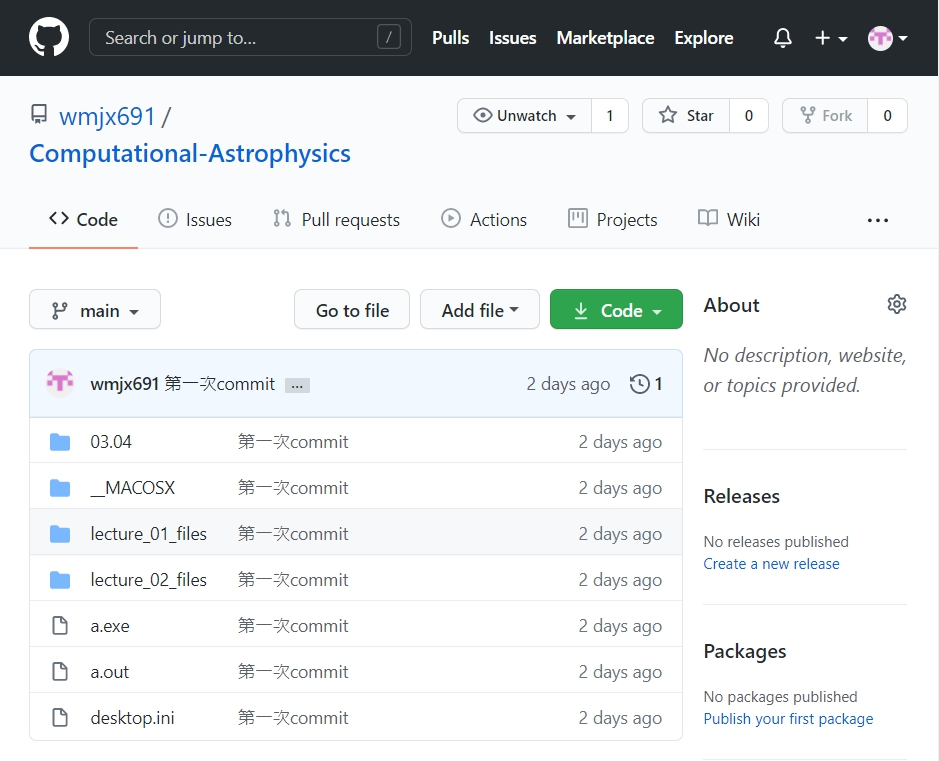
\includegraphics[scale=0.33]{github.jpg}
        \label{github}
    }
    \subfigure[folder which was tracked by git]{
        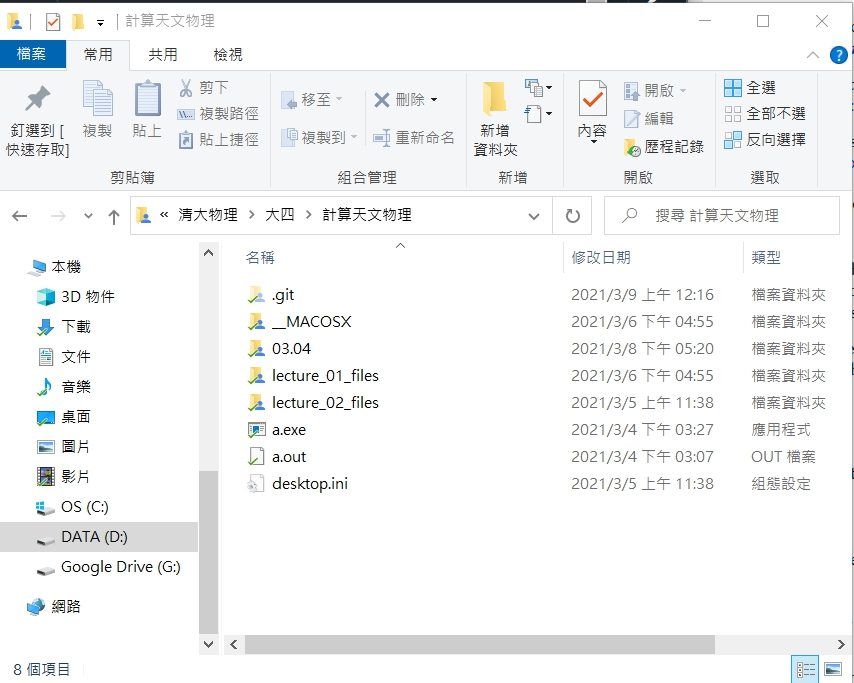
\includegraphics[scale=0.33]{git.jpg}
        \label{git} 
    }
    \caption{Using git to commit files onto github}
    \label{gversion}
\end{figure}
%Q2---------------------------------------------------------------------
\textbf{Q2 : Output of typing "which" and the version of gcc/gfortran}

Fig.\ref{which} is the output of the command "which gcc/gfortran".
I consider this command means where is location of this applicant be installed at.
%-------------------------------
\begin{figure}[h]
    \centering 
	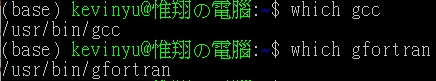
\includegraphics[scale=0.65]{which.jpg}
	\caption{Output of the command "which gcc/gfortran".} %圖片註解
	\label{which} %label 用這個就可以引用文章當中
\end{figure}
%-------------------------------

In Fig.\ref{gversion}, there are the version of them. gfortran was written as the repaired type of gcc. So I think that why them have the same version. \\
%-------------------------------
\begin{figure}[h]
    \centering
    \subfigure[gfortran]{
        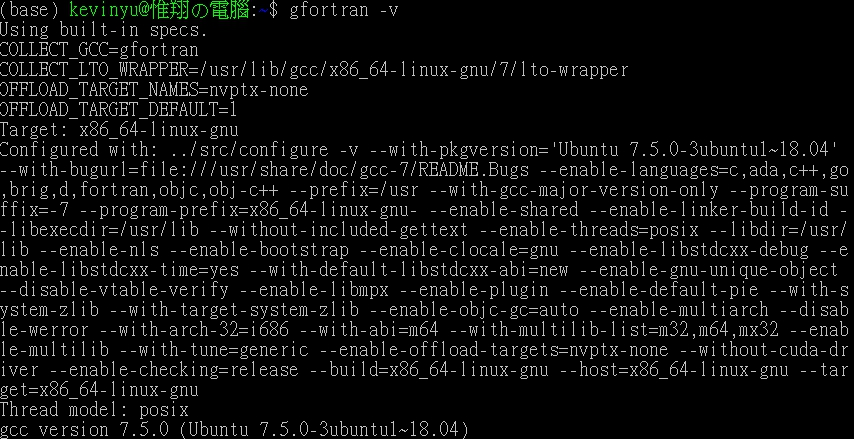
\includegraphics[scale=0.33]{gfortran.jpg}
        \label{gfortran}
    }
    \subfigure[gcc]{
        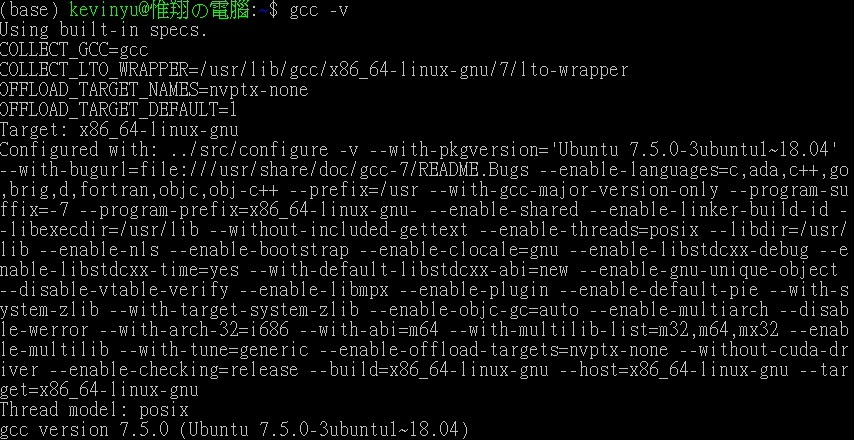
\includegraphics[scale=0.33]{gcc.jpg}
        \label{gcc} 
    }
    \caption{The version of application in my machine}
    \label{gversion}
\end{figure}

%-------------------------------
%Q3.4---------------------------------------------------------------------
\textbf{Q3 \& Q4 : The version of Python \& jupyter}\\

In Fig.\ref{Python}, the version of Python is 3.7.6, jupyter notebook is 6.0.3\\

%-------------------------------
\begin{figure}[h]
    \centering 
	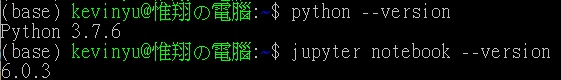
\includegraphics[scale=0.65]{python jyupter.jpg}
	\caption{The version of "python" \& "jupyter" in my computer.}
	\label{Python}
\end{figure}
%-------------------------------
%Q5---------------------------------------------------------------------
\textbf{Q5 : To install GNUPLOT \\}

My machine was installed WSL system, so gnuplot can not launch a new window to show the figure what I want to plot.I search the internet and find a website
\footnote{how to install gnuplot in WSL
\href{http://rocksaying.tw/archives/2018/wsl-run-linux-desktop-software.html}{http://rocksaying.tw/archives/2018/wsl-run-linux-desktop-software.html}}
teach how to fix this problem, and successfully launch a new window to show sin(x) in Fig.\ref{gnuplot}. 

%-------------------------------
\begin{figure*}[h]
    \centering 
	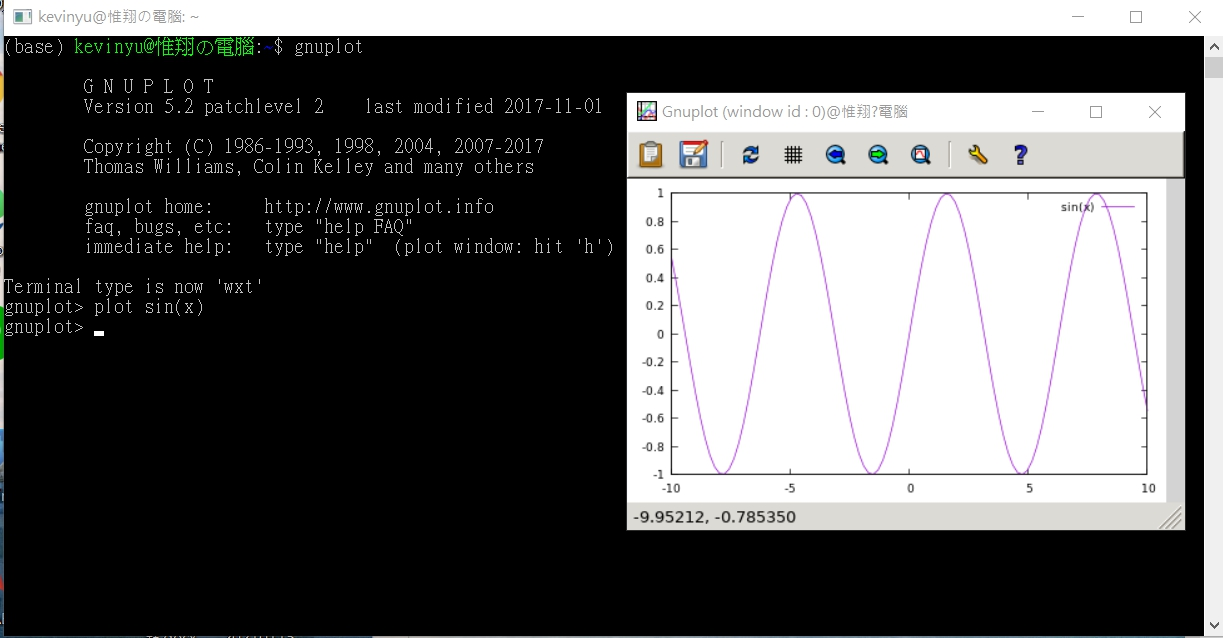
\includegraphics[scale=0.4]{gnuplot.jpg}
	\caption{plot sin(x) in WSL}
	\label{gnuplot}
\end{figure*}
%-------------------------------

\begin{CJK}{UTF8}{bsmi}
(But I also discussed with I-Fan(一璠), one of our classmate, his computer could show the window in the beginning when he installed gnuplot by following my reference website.
\end{CJK}
However, after reboost his computer, his WSL then could not output the plot...... we are still working on it.)

\end{document}